\section{Descripción}
El presente documento tiene como objeto exponer los requisitos, el funcionamiento  y cómo se usa el software que implementa la baliza RFID. \textit{Carrera con balizas contra-reloj}.

\section{Requisitos}
La baliza RFID necesita:
\begin{itemize}

   \item Un arduino Uno.
   \item Un lector RFID tipo \textit{RC522}. 
   \item Un diodo led, una resistencia y una \textit{protoboard}.
   \item Cables tipo \textit{jumpers} macho-macho y hembra-macho para realizar las conexiones.

\end{itemize}

El montaje hace referencia al \textit{pinout} de un Arduino Uno. Para otros modelos de Arduino el \textit{pinout} puede cambiar por lo que las siguientes indicaciones respecto a los interconexión de los pines podrían no ser válidas e incluso será necesario modificar el software.

En la \textit{protoboard} protoboard se conectarán el LED y la resistencia.  Uno de los extremos de la resistencia se conectará al pin 6 de Arduino Uno (pin 6 es donde se escribe la interrupción que recibirá el Nodo Central).  El otro extremo se conectará al extremo positivo del diodo LED.  Y el extremo negativo de éste se conectará al pin GND de la placa Arduino Uno.

El conexionado entre la placa Arduino Uno y el lector RFID deberá hacerse según reflejan las figuras siguientes:

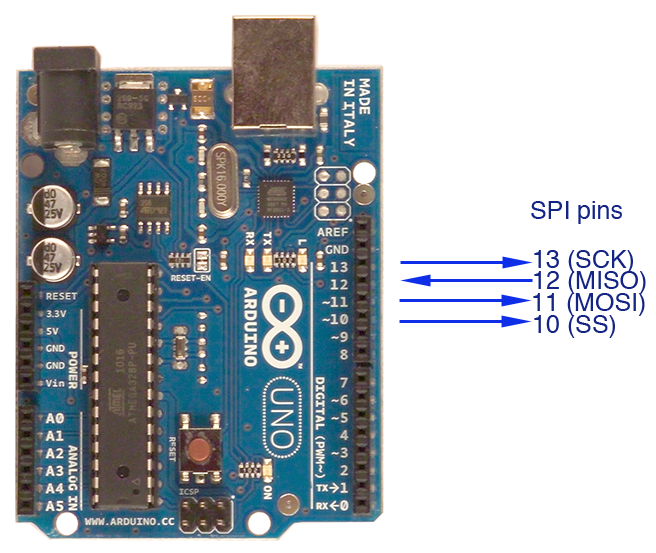
\includegraphics[scale=1,
         keepaspectratio]{./Figures/Arudiuno_SPI_pins.png}
         
        
     
         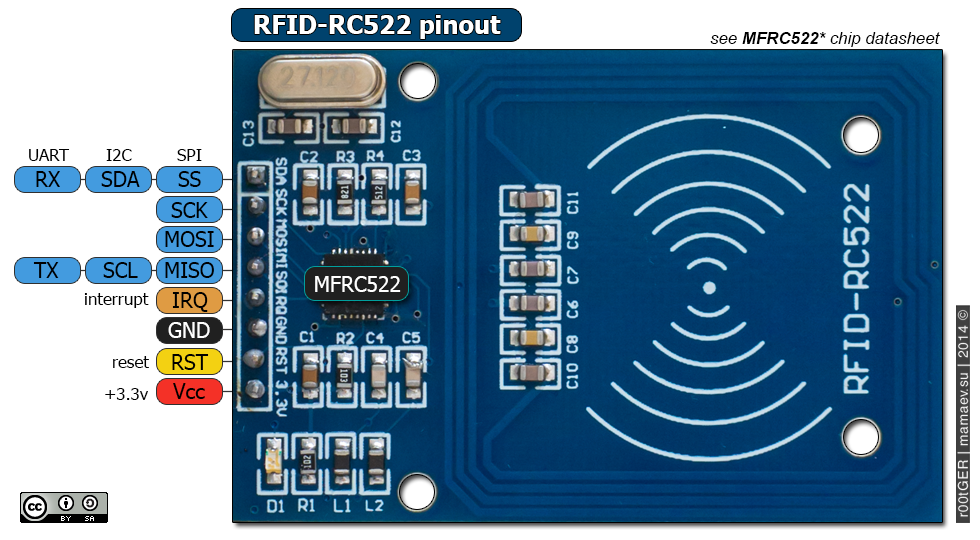
\includegraphics[scale=1,
         keepaspectratio]{./Figures/rfid-rc522-pinout.png}
   

Por otra parte será necesario descargar el código referente a la baliza RFID que se encuentra en el repositorio dentro del directorio \textit{Baliza-RFID/src} así como las librerías que se encuentran en el directorio \textit {Baliza-RFID/lib} a un directorio local desde donde se vaya a programar la placa Arduino Uno. Una vez descargado se compila con la herramienta de Arduino Uno y se sube el código binario a la placa.

\section{Especificaciones}
El juego constará de dos balizas RFIDs.  Cada baliza RFID, constituida por el conjunto \textit{Arduino Uno - Lector RFID - protoboard}, conecta el pin 6 al GPIO que recibe la interrupción del Nodo Central. 

El dron llevará acoplada una tarjeta RFID que podrá ser leída por los lectores RFIDs.
  
El juego comienza con un mensaje de bienvenida por parte del Nodo Central:
    \begin{description}
    		\item \hspace{10mm} ¡Bienvenido a la contra-reloj de drones!  
    		\item \hspace{10mm} Pulse el botón de 'start' para comenzar.
	\end{description}

Tras este mensaje, el usuario ya puede pulsar el botón de \textit{start} para comenzar el juego. Al pulsar el botón el jugador deberá colocar el dron en la posición de salida. Se mostrará por pantalla el siguiente mensaje:

    \begin{description}
    		\item \hspace{10mm} El juego ha comenzado. El dron puede despegar.
	\end{description}

El dron deberá dirigirse entonces a la primera baliza RFID intentando \textit{aterrizar} sobre ella.  Cuando lo consiga se mostrará el siguiente mensaje por pantalla:
    \begin{description}
    		\item \hspace{10mm} El tiempo del 1er 'checkpoint' ha sido: XXX milisegundos
	\end{description}
	
A continuación el dron deberá dirigirse a la segunda y última baliza RFID intentando nuevamente \textit{aterrizar} sobre ella.  Una vez lo consiga, el juego terminará y se mostrará el tiempo total que ha tardado el dron en realizar el circuito. 

A continuación el usuario podrá comenzar una nueva carrera volviendo a pulsar el botón de \textit{start}. El mensaje mostrado por pantalla será:

    \begin{description}
    		\item \hspace{10mm} Juego terminado. El tiempo total ha sido: XXX milisegundos
    		\item \hspace{10mm} Coloque el dron en la posición de salida y pulse el botón de 'start' para que de comienzo una nueva carrera.
	\end{description}	
